\section{Experiments}
\label{sec:experiments}

% ============================================================
% OUTLINE -- Experiments          target: ~1.1-1.25 pages
% Claims to land, in order:
%   (1) fine-tuning with the scaffolding helps (vs un-finetuned);
%   (2) small / open models become competitive with GPT Codex
%       5.3 under the SAME scaffolding;
%   (3) Qwen-30B is competitive with open-ended OpenHands at a
%       fraction of the token cost;
%   (4) the coverage term helps (lambda = 0 vs lambda > 0);
%   (5) the margin widens as the gold set grows / disperses.
% RESULTS ARE PARTIAL / IN PROGRESS -- scaffold the tables with
% placeholders and fill exact numbers before submission.
% ============================================================

\subsection{Setup}
\label{sec:setup-exp}

\paragraph{Datasets.}
The scorer is trained on a fixed subset of $5{,}000$ issues drawn
from the SWE-Bench train split \citep{jimenez2024swebench} and
evaluated on SWE-Bench Verified \citep{jimenez2024swebench} ---
the human-verified subset restricted to issues with unambiguous
patches --- and SWE-PolyBench \citep{chaudhari2025spider}, a
multilingual SWE-Bench-style benchmark spanning Python, Java,
JavaScript and TypeScript. Across all three splits we recover the
ground-truth function set $G_i$ from the PR commit that resolved
issue $i$: every function whose body the patch modifies is treated
as gold. Group construction and negative sampling at training time
follow Appendix~\ref{app:details}.

\paragraph{Backbones and baselines.}
The scorer is fine-tuned from Qwen2.5-Coder-3B-Instruct
\citep{hui2024qwen25codertechnicalreport}. As un-fine-tuned
reference points under the same scaffolding we report
Qwen2.5-Coder-14B-Instruct, Qwen3-Coder-30B-A3B-Instruct
\citep{yang2025qwen3}, and GPT-5.3
Codex\footnote{OpenAI's \texttt{gpt-5.3-codex} coding model,
accessed via the OpenAI API in 2025; the exact snapshot
identifier and access date will be pinned in the camera-ready
version.}. The first-stage retriever is either SWERankEmbed-Large
\citep{reddy2025sweranksoftwareissuelocalization} (dense) or BM25
(lexical), in both cases truncated to a top-$N$ pool with
$N{=}500$. The zero-shot retriever output and the un-fine-tuned
scorer under the same scaffolding act as ablation baselines.

\paragraph{Decoding and reproducibility.}
All scorer and agent calls use temperature $0$ and the API
default for top-$p$. Decoding is therefore deterministic up to
backend non-determinism, and rerunning a configuration on the
same inputs shifts Recall@$5$ by less than $1$ percentage point
in our measurements. Reported numbers are from single runs;
seeds and prompt templates are fixed across rows of a given
table to keep cross-row differences attributable to the
scaffolding rather than to sampling.

\subsection{Main Results}
\label{sec:main-results}

Table~\ref{tab:verified} reports $\text{Recall}@5$ on SWE-Bench
Verified ($N{=}500$) for the zero-shot retrievers, the
un-fine-tuned baselines, and our fine-tuned scorer, under both
first-stage retrievers. The block labelled \emph{w/o graph} is the
ablation in which Step~B is disabled (Section~\ref{sec:scaffold}),
so the loop reduces to window-only refinement; the \emph{full} block
runs the complete three-step round.

\begin{table*}[t]
\centering
\small
\setlength{\tabcolsep}{5pt}
\renewcommand{\arraystretch}{1.05}
\caption{Retrieval performance on SWE-Bench Verified
($N{=}500$). $\text{Recall}@5$ is reported separately under a
dense (SWERankEmbed-Large) and a lexical (BM25) first-stage
retriever. Token consumption is the total tokens per issue
(tokens/call $\times$ \#calls), averaged across the two
retrievers.
$^{*}$Zero-shot rows evaluate the raw retriever ranking at
$K{=}20$, since no LLM-based pruning is applied.}
\label{tab:verified}
\begin{tabular}{llccc}
\toprule
                  &                              & \multicolumn{2}{c}{$\text{Recall}@5$} &                  \\
\cmidrule(lr){3-4}
Method            & Model                        & Dense & BM25                          & Tokens (k)       \\
\midrule
\multirow{2}{*}{\emph{Zero-shot}}
                  & SWERankEmbed-Large           & $0.35^{*}$ & --                       & --               \\
                  & BM25                         & --         & $0.36^{*}$               & --               \\
\midrule
\multirow{5}{*}{\emph{w/o graph}}
                  & GPT-5.3 Codex                & $0.51$ & --                           & $63$           \\
                  & Qwen2.5-14B-Instruct         & $0.26$ & $0.29$                       & $73$           \\
                  & Qwen2.5-Coder-14B-Instruct   & $0.35$ & $0.35$                       & $69$           \\
                  & Qwen3-Coder-30B-A3B-Instruct & $0.50$ & $0.50$                       & $70$           \\
                %   & \quad + Qwen2.5-Coder-3B scorer (ours) & $\mathbf{0.45}$ & --       & $\mathbf{33}$  \\
\midrule
\multirow{4}{*}{\shortstack[l]{\emph{w/ graph, w/o scorer}}}
                  & GPT-5.3 Codex                & $0.56$ & $0.56$                       & $204$          \\
                  & Qwen2.5-14B-Instruct         & $0.36$ & $0.36$                       & $204$          \\
                  & Qwen2.5-Coder-14B-Instruct   & $0.44$ & $0.42$                       & $198$          \\
                  & Qwen3-Coder-30B-A3B-Instruct & $0.54$ & $0.55$                       & $271$          \\
\cdashline{1-5}
\emph{w/graph, w/ scorer}  & \multirow{2}{*}{Qwen3-Coder-30B-A3B-Instruct} & \multirow{2}{*}{$\mathbf{0.55}$} & \multirow{2}{*}{--}    & \multirow{2}{*}{$\mathbf{35}$}  \\
\emph{Ours} & & & & \\
\bottomrule
\end{tabular}
\end{table*}


Three observations stand out. \emph{First}, the zero-shot
retrievers plateau near $0.35$ Recall@5; the LLM-driven refinement
loop closes a substantial part of that gap even without any
training. \emph{Second}, adding graph exploration (Step~B) lifts
every model in the table, with the largest absolute jumps on
small backbones: Qwen2.5-Coder-14B-Instruct rises from $0.354$ to
$0.435$ under BM25 retrieval, and Qwen3-Coder-30B-A3B-Instruct
moves from $0.502$ to $0.549$. Total token consumption rises
roughly $3\times$ with exploration, driven by the higher call
count even as per-call context shrinks. \emph{Third}, the smallest
open backbones still trail GPT-5.3 Codex (which reaches $0.559$
under the full scaffolding), motivating the fine-tuned scorer
whose results occupy the last row.

\paragraph{Standalone scorer analysis.}
To isolate the scorer from the multi-round scaffolding,
Figure~\ref{fig:scorer-func-recall} reports function-level
recall on SWE-PolyBench under a single-pass windowed protocol:
the first-stage retriever returns the top $\text{PS}{=}100$
candidates, the scorer ranks a window of $K{=}20$, and the
top-$L{=}5$ by score are selected. The fine-tuned 3B
scorer dominates both 0.5B variants and closes most of the gap
to GPT-5.3 Codex across languages despite being two orders of
magnitude smaller. File-level recall and a calibration
diagnostic ($p_{gt}$ vs.\ $p_{\neg gt}$) under the same protocol
are deferred to Appendix~\ref{app:results}.

\begin{figure}[t]
\centering
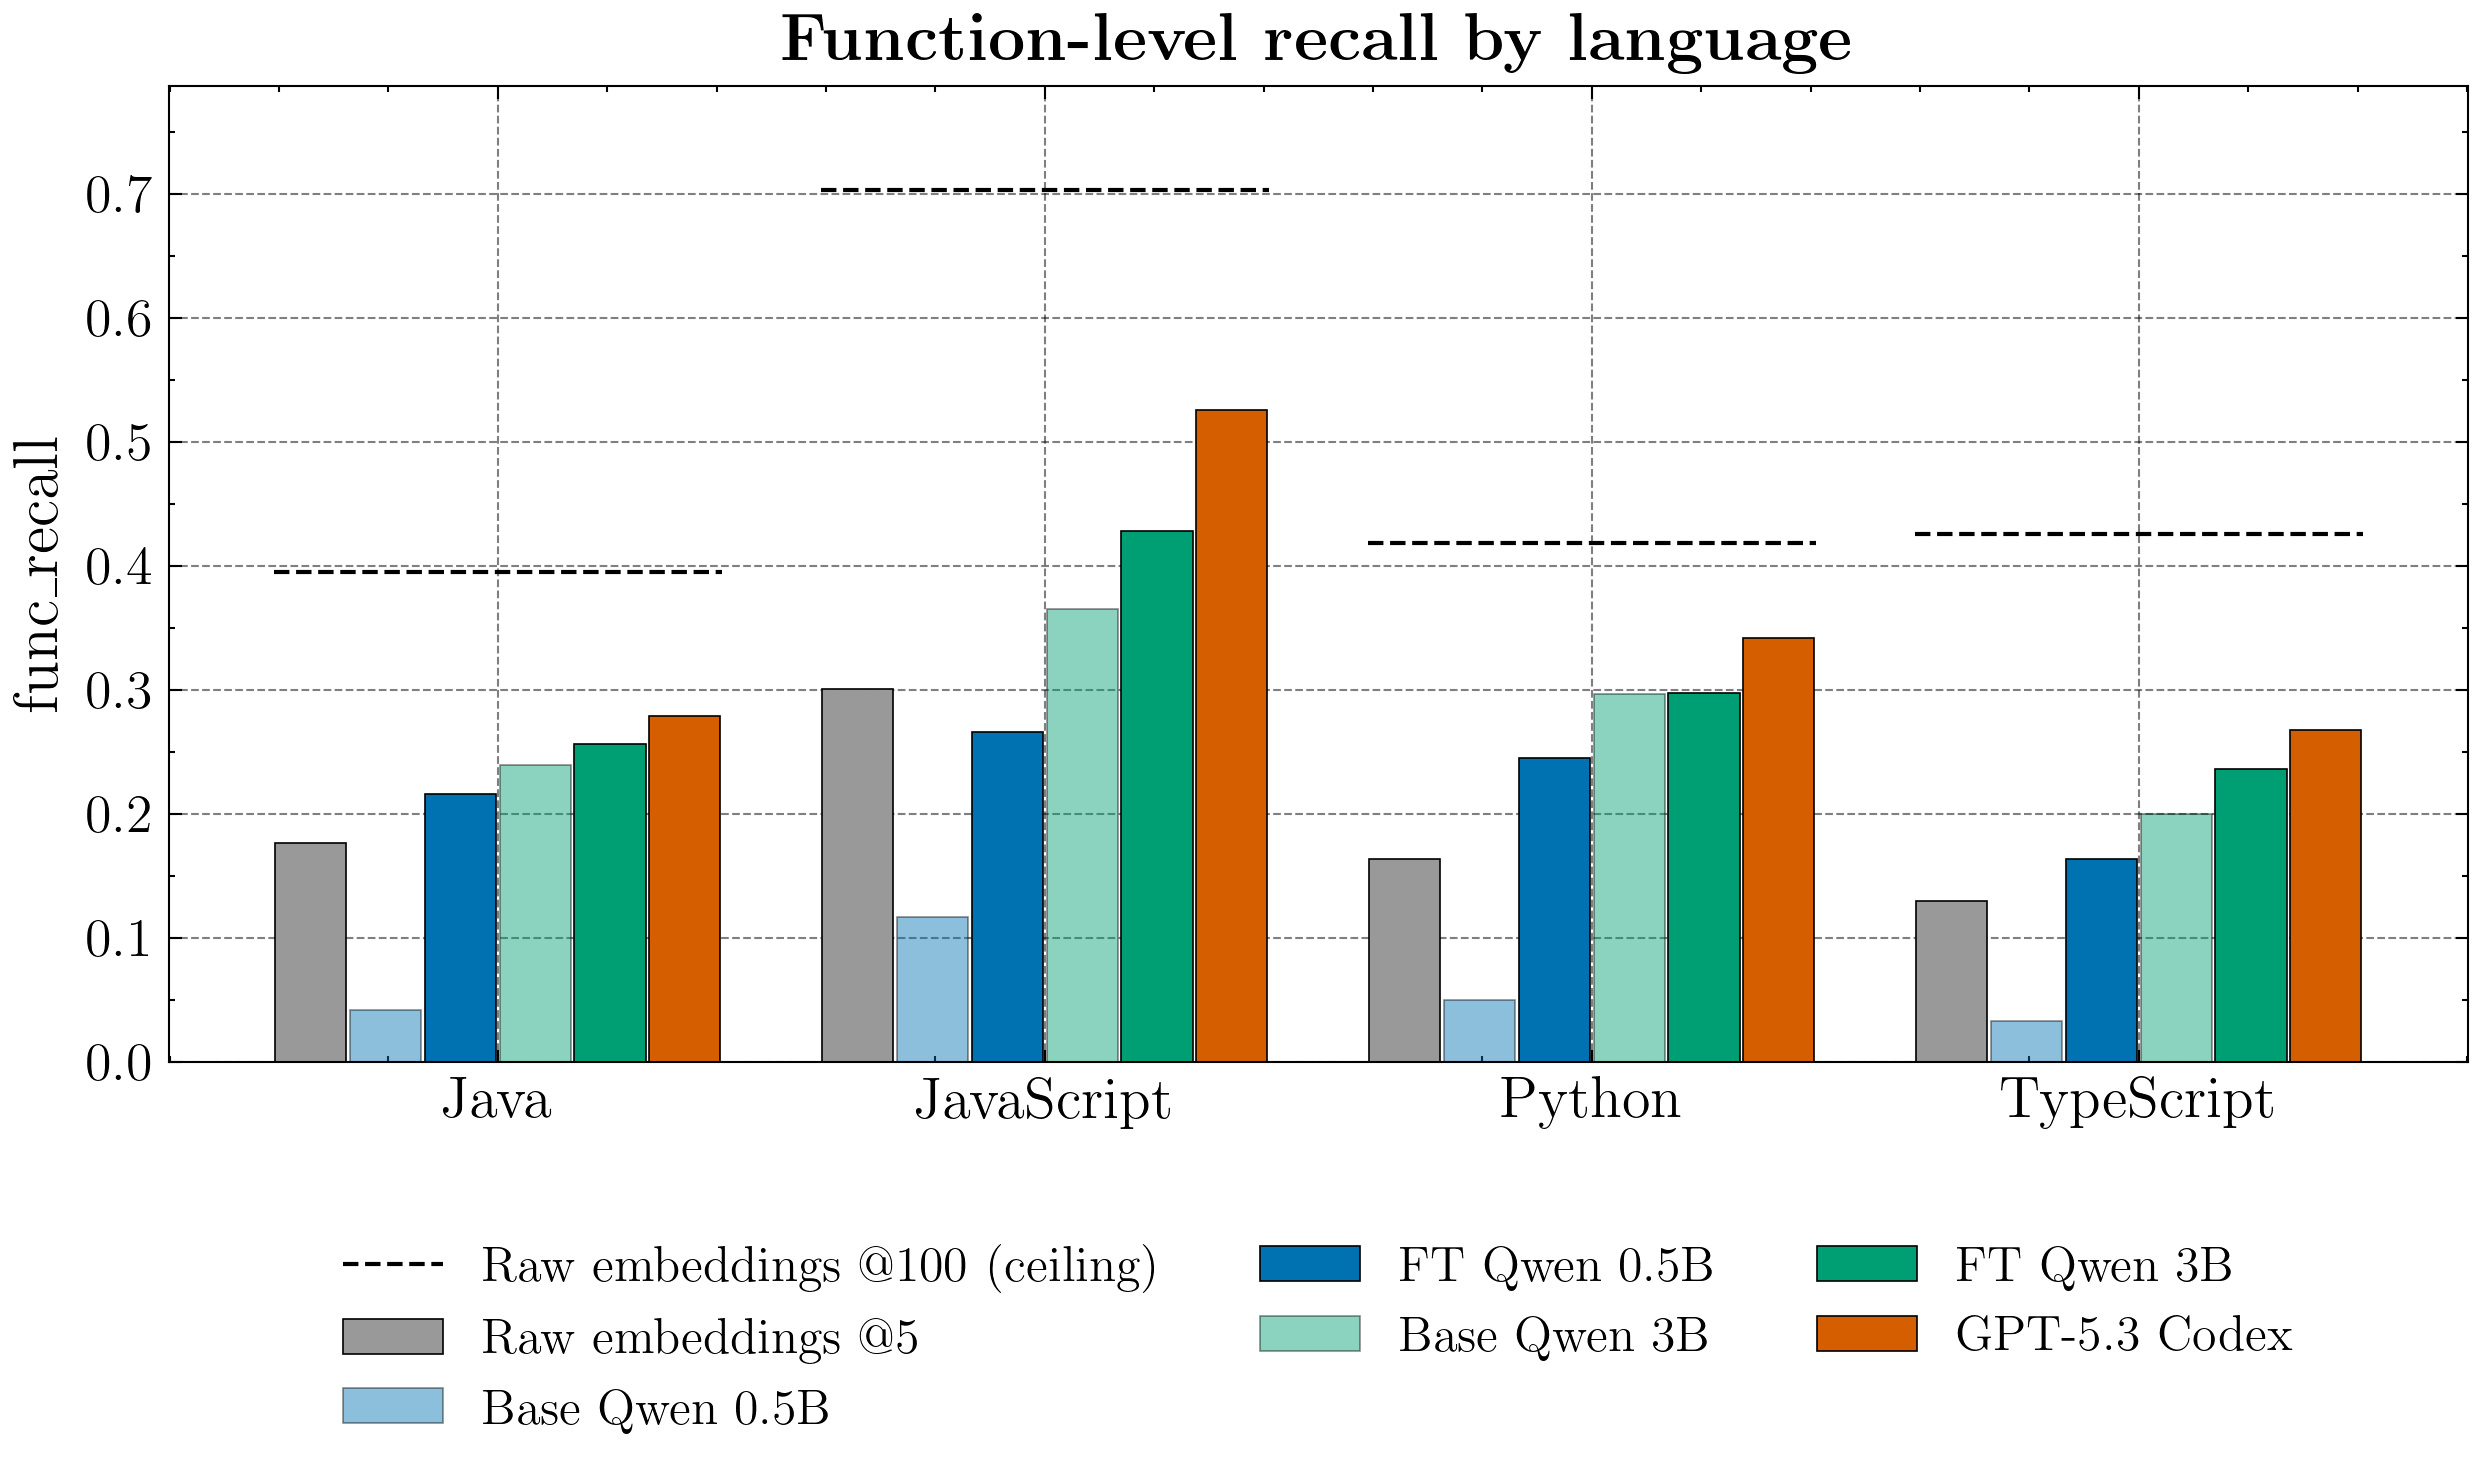
\includegraphics[width=\columnwidth]{imgs/reranker_func_recall.png}
\caption{Per-language function-level recall on SWE-PolyBench
under a windowed scorer protocol (pool size
$\text{PS}{=}100$, candidate window $K{=}20$, top-$L{=}5$). The
dashed line is the retrieval ceiling at $\text{PS}{=}100$.
Comparisons include the raw embedding ranker at $L{=}5$, base
and fine-tuned Qwen2.5-Coder 0.5B/3B-Instruct, and GPT-5.3
Codex. The fine-tuned 3B scorer dominates the 0.5B variants
and trails GPT-5.3 Codex by $2$--$10$ points across languages;
JavaScript shows the largest residual gap, where GPT-5.3 Codex
benefits most from its longer context.}
\label{fig:scorer-func-recall}
\end{figure}

\paragraph{End-to-end results on SWE-PolyBench.}
Table~\ref{tab:swepoly-java-python} reports end-to-end Recall@5
and Accuracy@5 on the SWE-PolyBench Java and Python splits,
where Accuracy@$K := \frac{1}{N}\sum_i \mathbb{1}[G_i \subseteq
\hat{L}_i]$ is the fraction of issues for which \emph{every}
gold function is recovered (i.e.\ perfect recall), comparing the scaffolding without graph
exploration (Step~B disabled) against the full scaffolding with
our fine-tuned scorer. The full scaffolding improves both
metrics on both languages: on Java, GPT-5.3 Codex gains $+5$
recall and $+5$ accuracy points; on Python, Qwen3-Coder-30B
gains $+5$ recall and $+4$ accuracy points and overtakes the
GPT-5.3 Codex baseline. Token consumption stays comparable to
the no-graph variant, so the gains come essentially free of
extra compute.

The Python ordering deserves a closer look: Qwen3-Coder-30B
overtakes GPT-5.3 Codex not because of better retrieval, but
because GPT-5.3 Codex triggers the early-stop flag too
aggressively. On the $120$ Python issues where GPT-5.3 Codex
ended the loop early, its Recall@5 is $0.476$, whereas Qwen3
running the full round budget on the \emph{same} issues reaches
$0.529$ --- a $+5.3$-point gap that comes entirely from the
exploration rounds GPT chose to skip. The recall deficit is
therefore a confidence-calibration artefact at Step~C, not a
shortcoming of the scorer or the retriever.

\begin{table*}[t]
\centering
\small
\setlength{\tabcolsep}{5pt}
\renewcommand{\arraystretch}{1.05}
\caption{Retrieval performance on SWE-PolyBench Java and Python
under two Step-C agents (GPT-5.3 Codex and
Qwen3-Coder-30B-A3B-Instruct). Recall@5 and Accuracy@5 (perfect
recall) are reported after filtering out instances with empty
function-level GT and using denominator
$|GT \cap \mathrm{graph\_functions}|$. ``--'' marks a run we
have not executed. Token consumption is the total tokens per
issue (tokens/call $\times$ \#calls), averaged across kept
instances.}
\label{tab:swepoly-java-python}
\begin{subtable}{0.49\textwidth}
\centering
\setlength{\tabcolsep}{4pt}
% \caption*{Java (kept $= 158$ / $165$)}
\caption*{Java}
\begin{tabular}{lccc}
\toprule
Model                          & Rec@5 & Acc@5 & Tokens (k) \\
\midrule
\multicolumn{4}{l}{\emph{w/o graph (Step B disabled)}} \\
GPT-5.3 Codex                  & $0.38$ & $0.22$ & $21.7$ \\
Qwen3-Coder-30B-A3B            & $0.35$ & $0.20$ & $27.8$ \\
\midrule
\multicolumn{4}{l}{\emph{Full, ours (Qwen2.5-Coder-3B scorer)}} \\
GPT-5.3 Codex                  & $\mathbf{0.43}$ & $\mathbf{0.27}$ & $\mathbf{19.1}$ \\
Qwen3-Coder-30B-A3B            & $0.37$ & $0.20$ & $26.8$ \\
\bottomrule
\end{tabular}
\end{subtable}
\hfill
\begin{subtable}{0.49\textwidth}
\centering
\setlength{\tabcolsep}{4pt}
% \caption*{Python (kept $= 182$ / $199$)}
\caption*{Python}
\begin{tabular}{lccc}
\toprule
Model                          & Rec@5 & Acc@5 & Tokens (k) \\
\midrule
\multicolumn{4}{l}{\emph{w/o graph (Step B disabled)}} \\
GPT-5.3 Codex                  & --     & --     & --     \\
Qwen3-Coder-30B-A3B            & $0.40$ & $0.29$ & $38.1$ \\
\midrule
\multicolumn{4}{l}{\emph{Full, ours (Qwen2.5-Coder-3B scorer)}} \\
GPT-5.3 Codex                  & $0.42$ & $0.31$ & $\mathbf{30.9}$ \\
Qwen3-Coder-30B-A3B            & $\mathbf{0.45}$ & $\mathbf{0.33}$ & $46.4$ \\
\bottomrule
\end{tabular}
\end{subtable}
\end{table*}

% \subsection{Does the Coverage Term Help?}
% \label{sec:ablation}
% - The key ablation: lambda = 0 (BCE only) vs lambda = 0.2
%   (BCE + coverage). Report the recall@L delta -- this is THE
%   objective-paper result.
% - Diagnostics (one line here, rest -> appendix): mean p on
%   gold vs non-gold; fraction of golds landing in the top-L.
%   (~0.2 page)

% \subsection{Efficiency and Scaling}
% \label{sec:efficiency}
% - FIGURE 2: token cost. Per-call and total tokens vs
%   OpenHands; bounded vs unbounded trajectory length; wall-
%   clock saved. Plot with SciencePlots (project .venv, PDF).
% - Scaling: recall@L vs number-of-gold-nodes and vs gold
%   graph-spread -- a widening margin over a ranking baseline
%   (SweRank). This is the make-or-break analysis.
% - TRIAGE: 4 pages cannot comfortably hold both an efficiency
%   figure and a scaling figure. Put ONE in the body (the
%   scaling figure is the stronger novelty signal) and move the
%   other to Appendix C, or render efficiency as a small table.
%   (~0.25-0.3 page)
